\section{Durchführung}
\label{sec:Durchfuehrung}
Für den Versuch wird als ANodenmaterial Kupfer verwendet und über eine Blende der Röntgenstrahl auf das Material gelenkt.
Die Elektronen werden mit einer Beschlenigungsspannung von  $35 \text{keV}$ beschleunigt.
Es lassen sich sowohl der verwendete LiF Kristall als auch das Geiger Müller Zählrohr im Bezug auf den Strahl drehen.
Für den letzten Teil des Versuchs lässt sich zwischen der Blende und dem Kristall eine Probe anbringen um die Absorption zu messen.
\begin{figure}
    \centering
    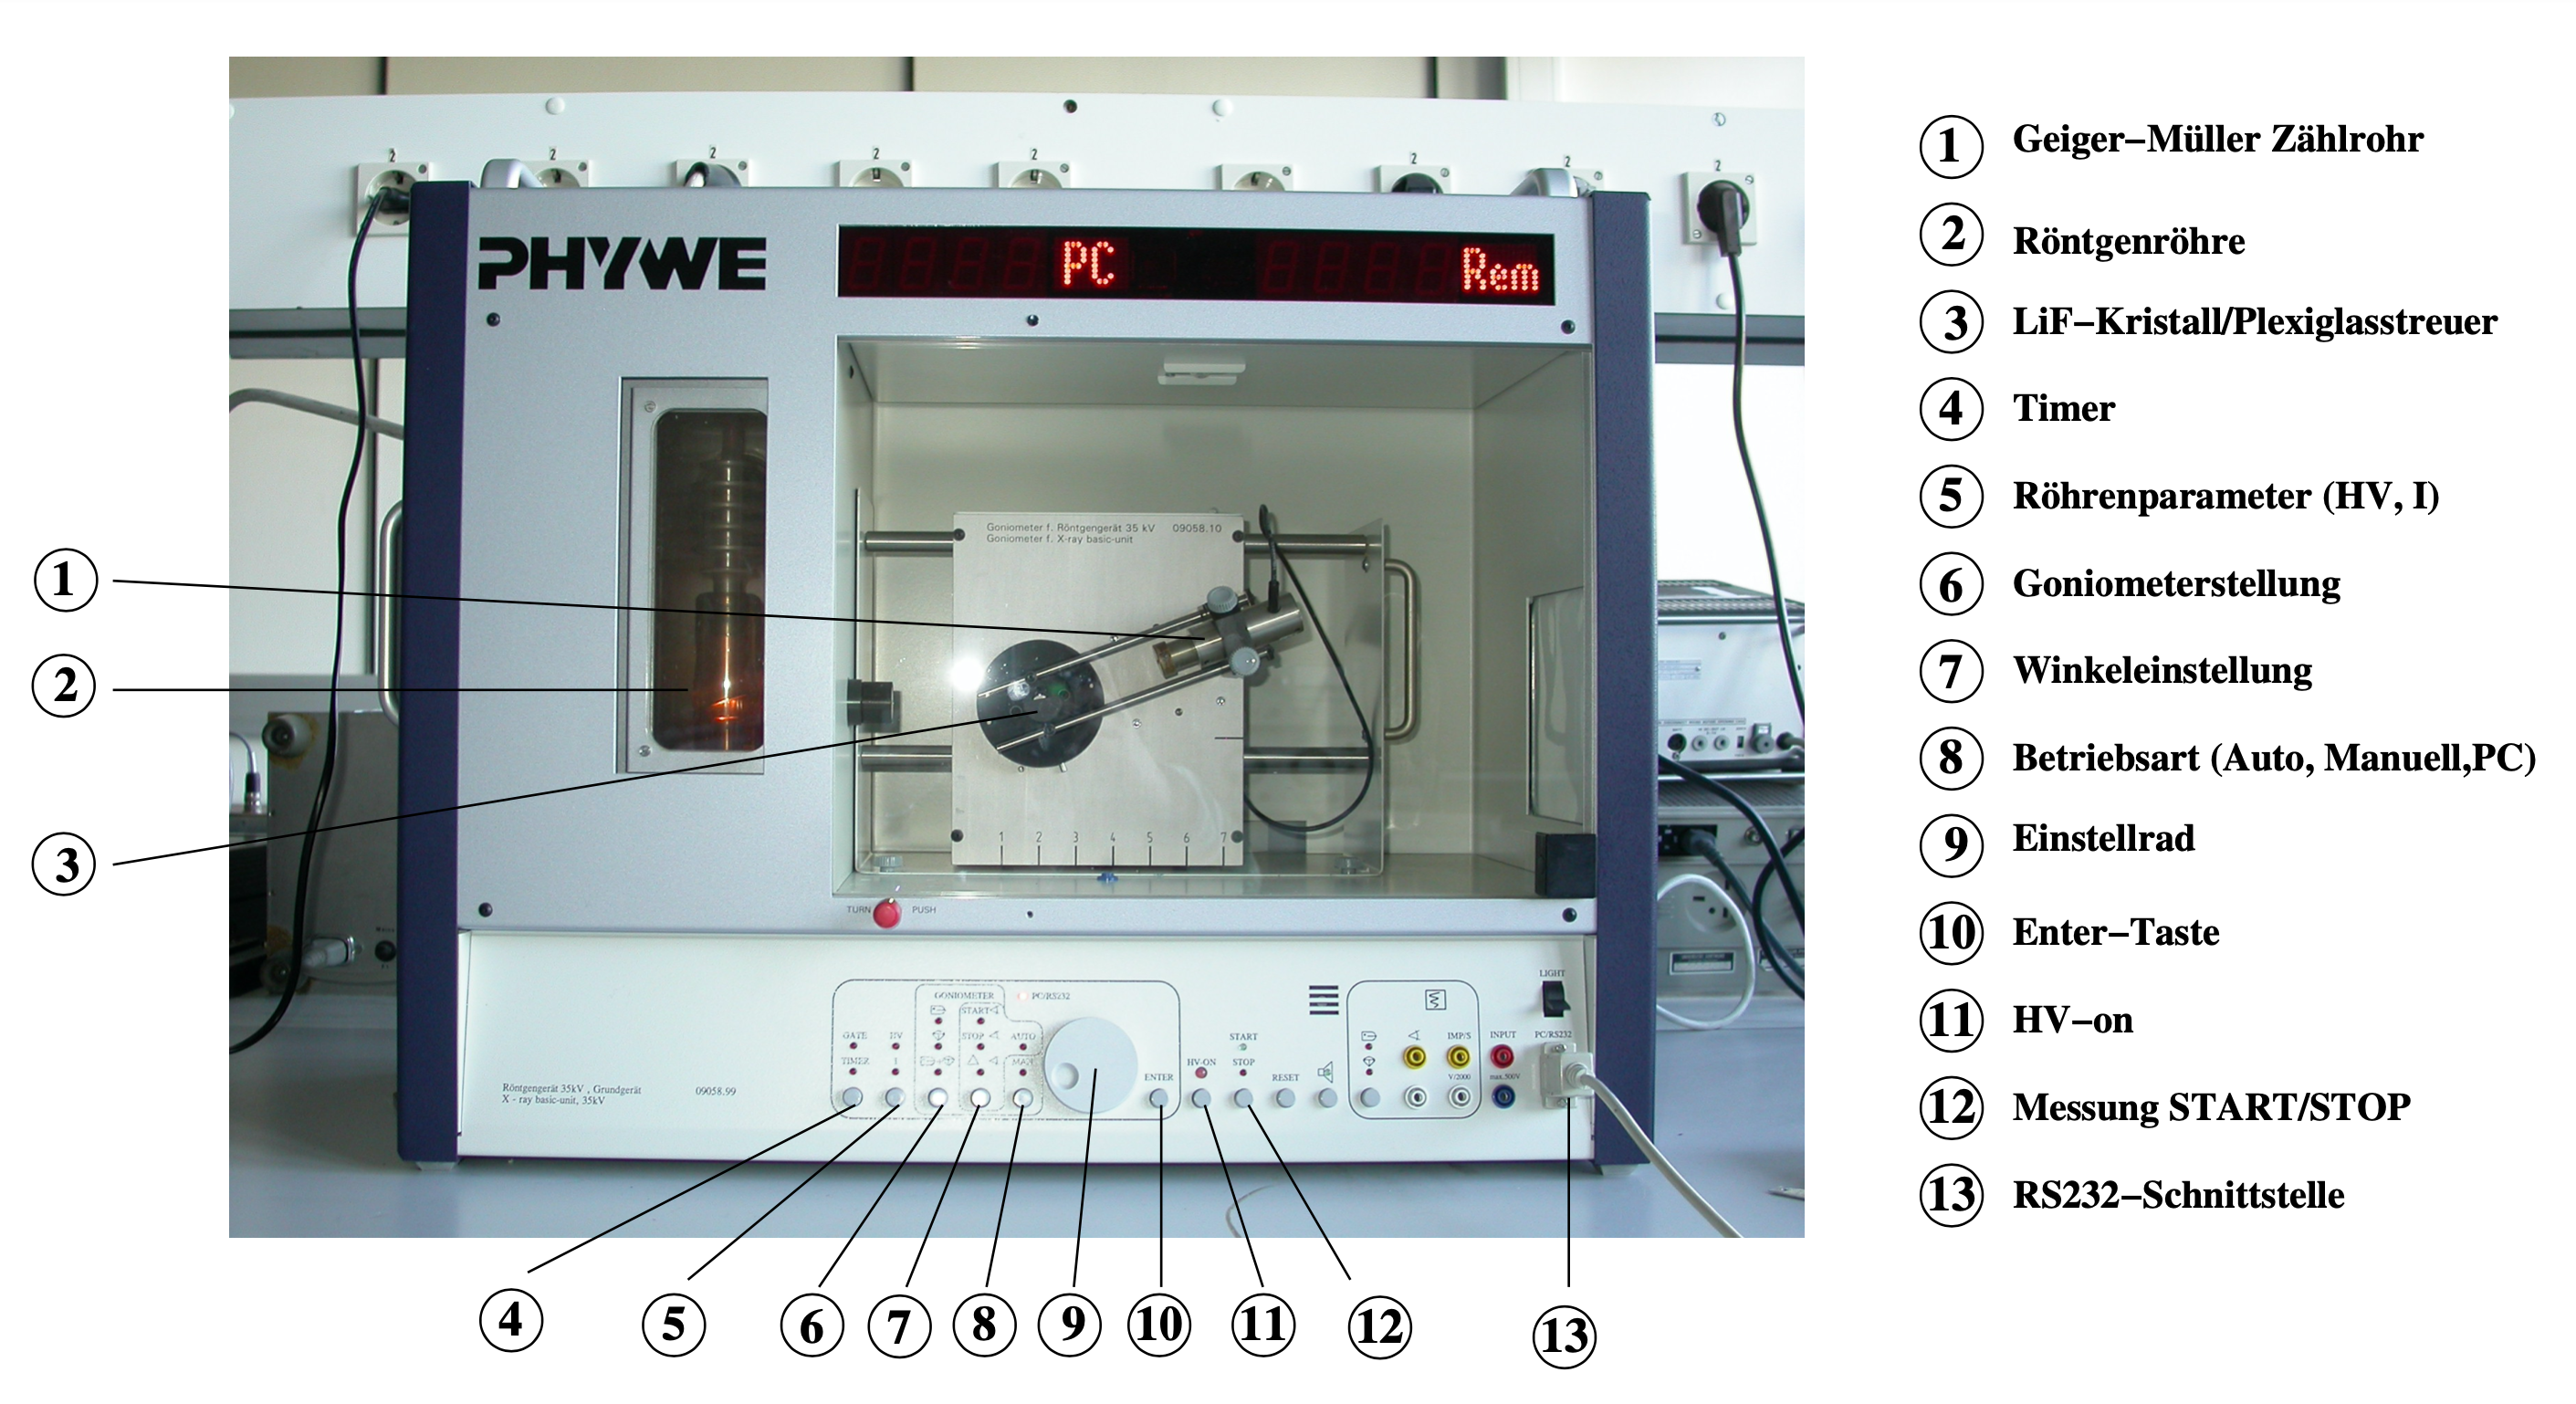
\includegraphics[width=0.7\textwidth]{bilder/Versuchsaufbau.png}
    \caption{Ein Foto des Versuchsaufbaus mit Beschriftung der Komponenten. (Quelle \cite{Anleitung})}
    \label{fig:Versuchsaufbau}
\end{figure}

\subsection{Braggbedingung überprüfen}
Für die Überprüfung der Braggbedingung wird der LiF Kristall in einen festen Winkel $\alpha = 14°$ zum Photonenstrahl gebracht.
Nun wird das Geiger Müller Zählrohr Über das Winkelintervall von 26° bis 30° in $\Delta \alpha = 0,1°$ Schritten mit einer Integrationszeit von $\Delta t = 5 \text{s}$ gedreht.
Aus den Werten lässt sich das Intensitätsmaximum auslesen und mit der Braggbedingung vergleichen.
\subsection{Kupfer Emissionsspektrum}